\section{Contexte \& Démarche}
\subsection{Contexte}
Le projet se déroule dans une équipe d'intégration.
Le projet est cadré par mon encadrant de stage qui désigne les objectifs du projet.
Pour le réaliser, je suis accompagné d'un référent technique.

On a une structure transverse, le travail est autonomie, mais j'ai le support de toute l'équipe.

\subsection{Démarche}
Au sein de la VSCT, on met beaucoup de points sur la méthode agile et la discipline "Devops"(lexique. \ref{lexi:devops}).
Dans cette équipe, on applique un "Kanban"(lexique. \ref{lexi:kanban}) pour l'organisation des travaux.
Comme sur la figure (fig. \ref{fig:kanban}), chaque membre dispose d'une ligne sur le tableau et chaque ligne est découpé en trois parties: "TODO", "EN-COUR" et "DONE" qui correspondant aux tâches à faire, tâche en train de faire et tâches réalisés.
Les espaces laissés à gauche sont pour des idées qu'on va pêut-être planifier un jour.

\begin{figure}[ht]
\centering
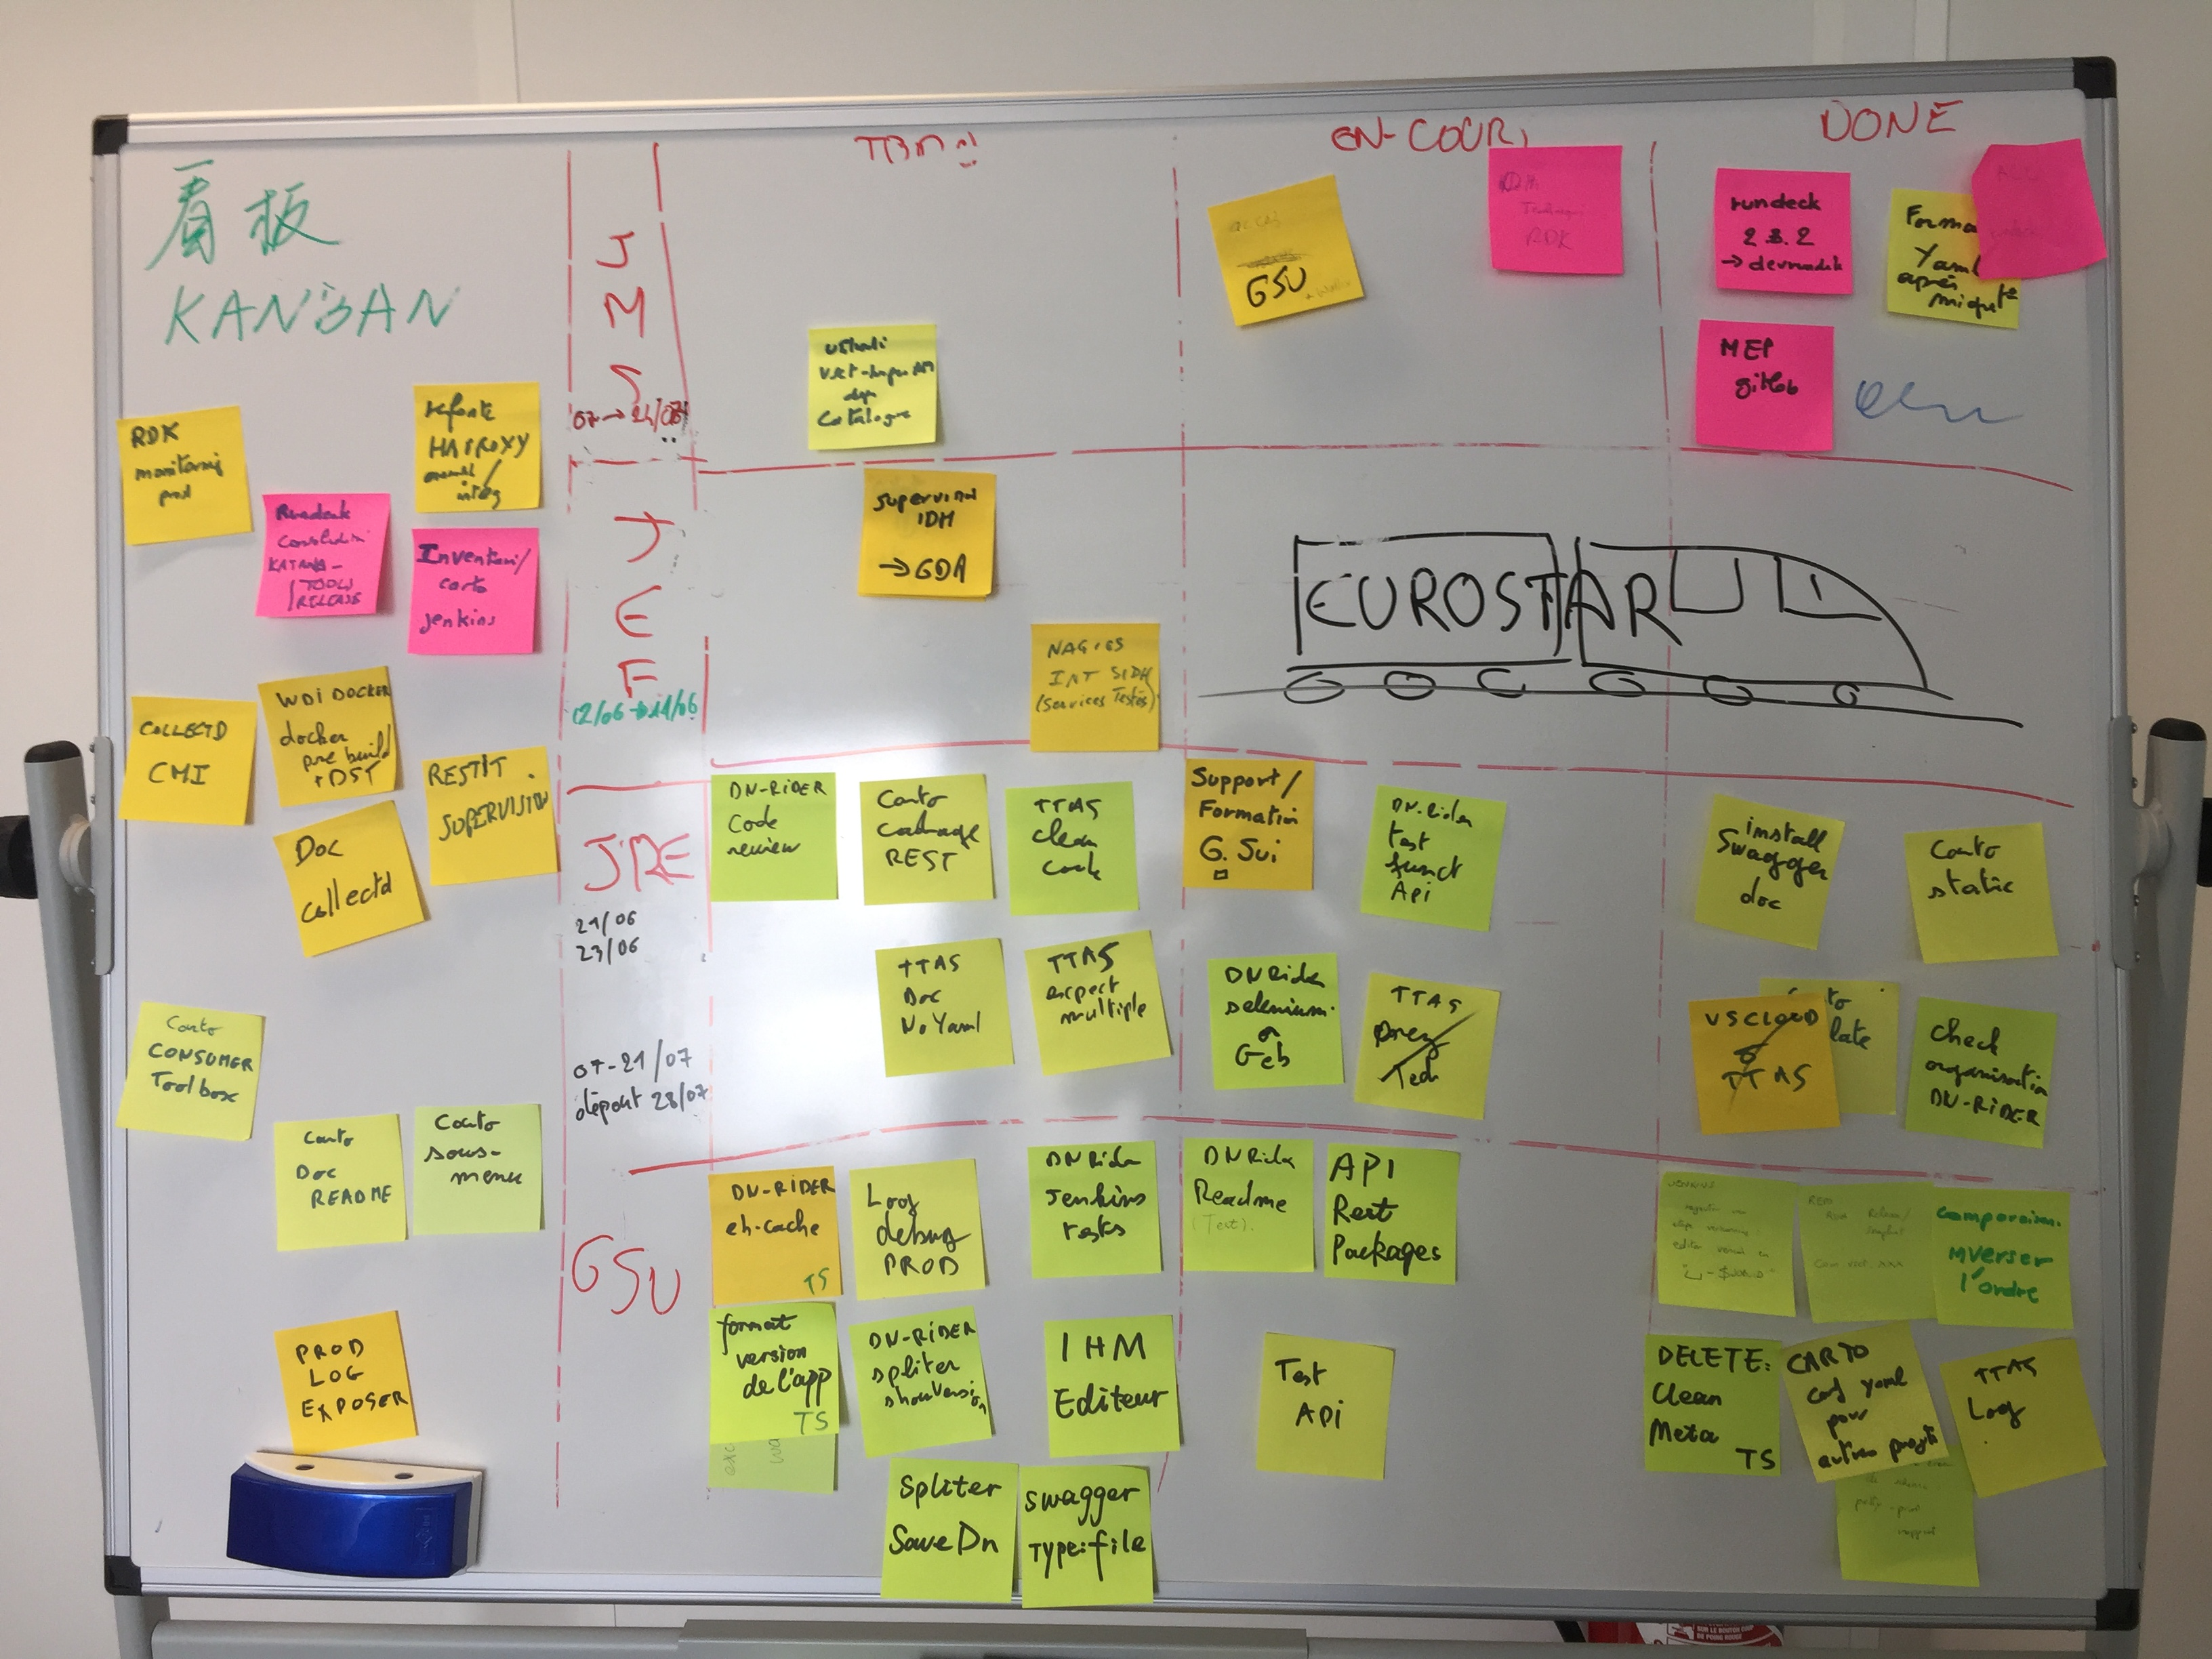
\includegraphics[width=0.9\textwidth]{kanban}
\caption{Kanban}
\label{fig:kanban}
\end{figure}

On applique la "post-it theory"(lexique. \ref{lexi:post_it_theory}).
Les post-its sont classés par leurs colleurs, les plus profonds correspondants aux tâches plus importants.
Certaines cartes sont marquées "TS" (Technic Story) dessus, c'est-à-dire que c'est un petit soucis technique qui n'est pas urgent à être résolu, on a une grande liberté de l'organiser selon notre convenance.

Normalement on fait  deux fois par semaine la revue du Kanban pour garder le rythme.
Chaque fois mes tuteurs valident ce que j'ai réalisé et m'aident à planifier les tâches suivantes.

Les codes sources sont géré en git et stocké sur Gitlab. Au bout d'un mois et demi, on a la première version de l'application et on commence à faire intégration continue en utilisant Jenkins pipeline.
Chaque fois qu'il y a un commit sur la branche "master", l'application seront déploiée toute seule.

\clearpage
